\subsubsection{Raman Spectroscopy with Graphene}

\begin{figure}[!h]
  \centering
  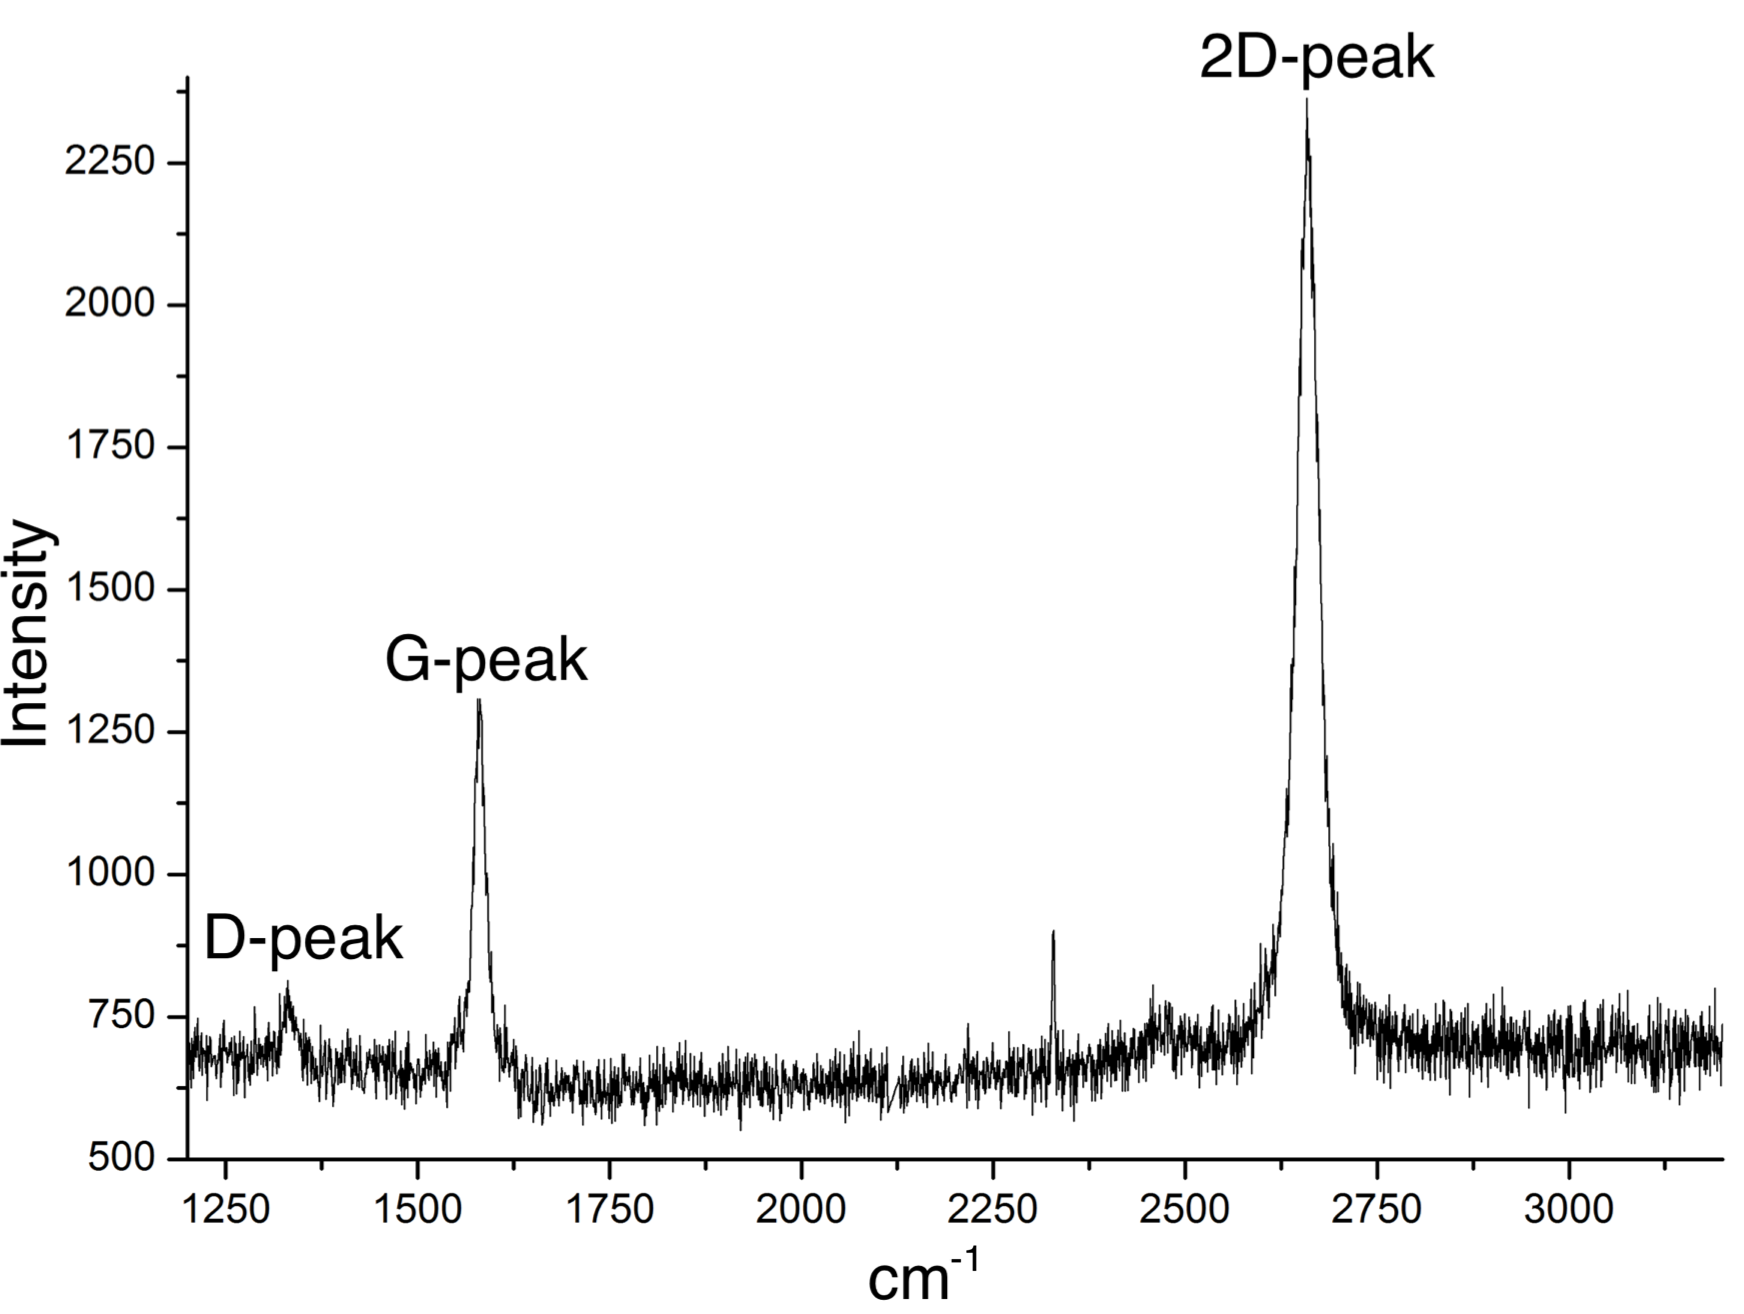
\includegraphics[width=0.7\textwidth]{./images/graphene-raman.png}
  \caption{\textbf{(a)} Calculated phonon dispersion relation of graphene along the $\Gamma$-$K$-$M$-$\Gamma$-direction with six phonon branches (Figure adapted from Malard et al. 2009\mcite). \textbf{(b)} The Raman spectrum of graphene showing the $D$, $G$ and $2D$ modes.(adapted from \mcite, \note{add new image here}).}
\end{figure}

\note{phonon dispersion in relation to electromagnetic dispersion. leads to 3 major peaks in graphene (one is a defect)}

\begin{figure}[!h]
  \centering
  \begin{subfigure}{0.7\textwidth}
    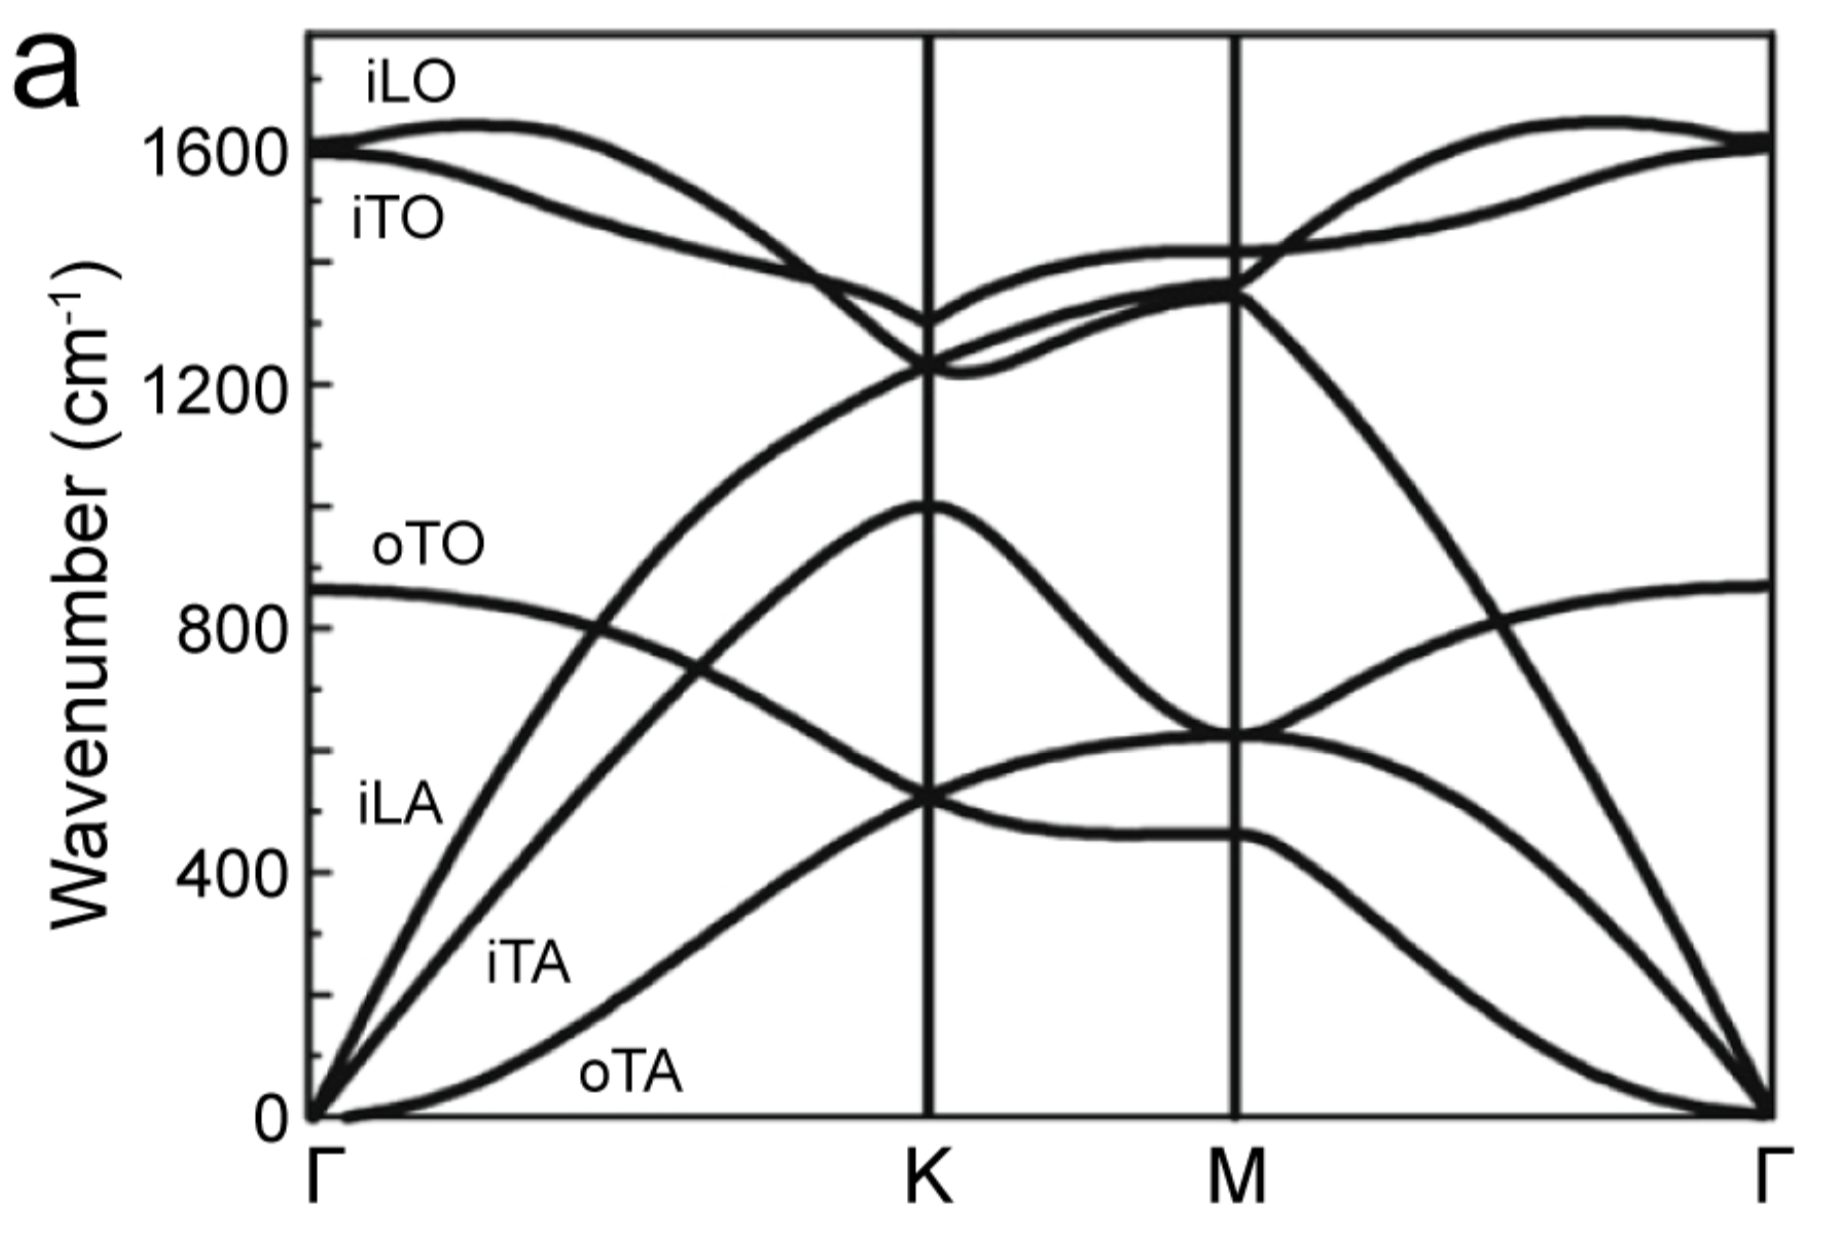
\includegraphics[width=\textwidth]{./images/phonon-modes.png}
  \end{subfigure}
  ~
  \begin{subfigure}{0.25\textwidth}
    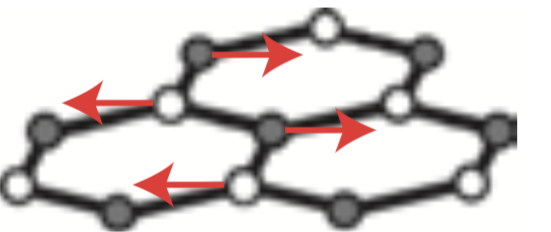
\includegraphics[width=\textwidth]{./images/g-mode-phonon.png}
    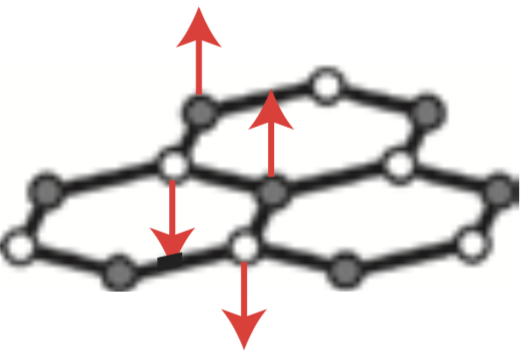
\includegraphics[width=\textwidth]{./images/g-mode-phonon-2.png}
    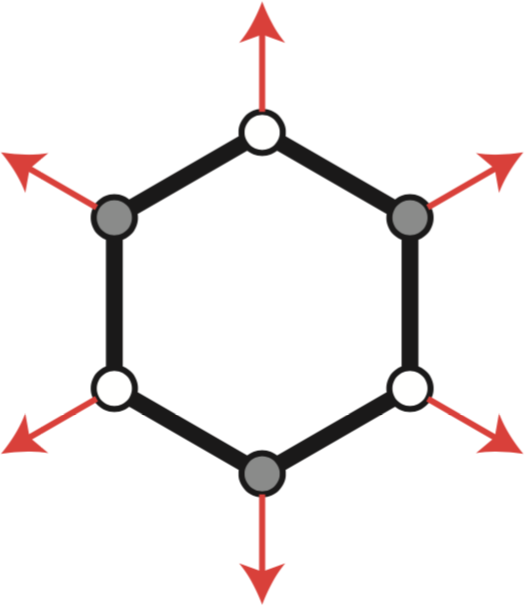
\includegraphics[width=\textwidth]{./images/2d-mode-phonon.png}
  \end{subfigure}
  \caption{\textbf{(a)} $\Gamma$ point displacement pattern for graphene, causing the $G$-peak in graphene's Raman spectrum. \textbf{(c)} Displacement at $K$ causing the $2D$-peak in graphene's Raman spectrum.}
\end{figure}

\begin{figure}[!h]
  \centering
  \begin{subfigure}{0.2\textwidth}
    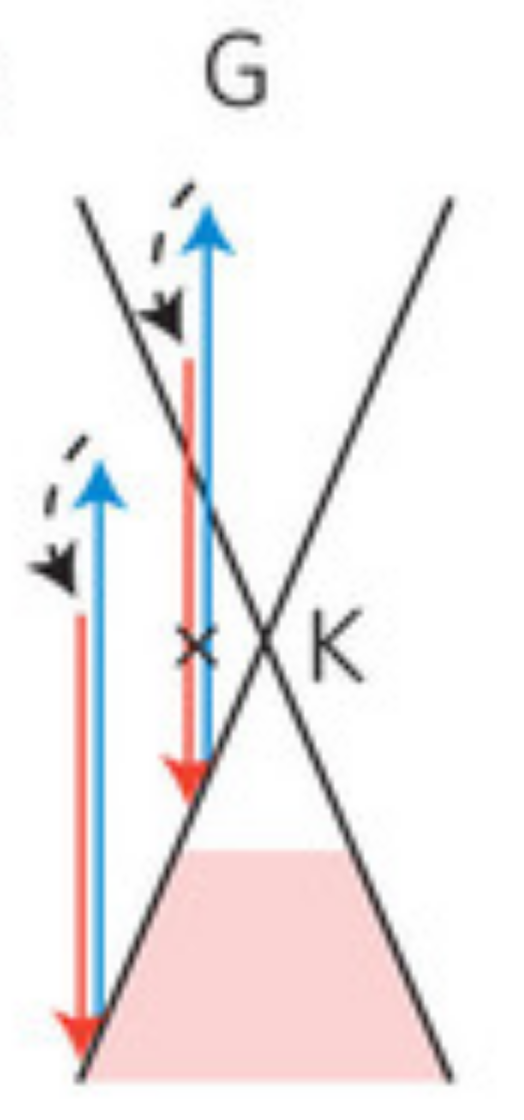
\includegraphics[width=\textwidth]{./images/g-mode.png}
  \end{subfigure}
  ~
  \begin{subfigure}{0.45\textwidth}
    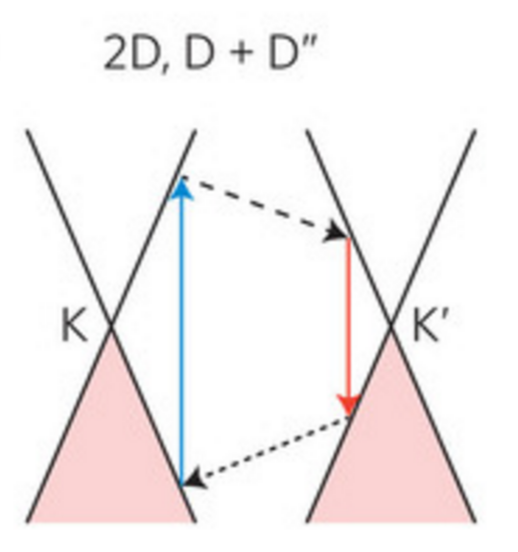
\includegraphics[width=\textwidth]{./images/2d-mode.png}
  \end{subfigure}
  \caption{Raman scattering processes for the $G$ and $2D$ peak of graphene. The band structure close to the K points is approximated as cones. \textbf{(a)} A photon is absorbed (blue arrow), scatters with a phonon (dashed arrow) and then is emitted with a lower frequency (red arrow), causing the $G$ peak in graphenes Raman spectrum. \textbf{(b)} A photon is absorbed (blue arrow), then scatters with two phonons (dashed arrows) and is emitted at a lower frequency (red arrow). This is the most prominent feature of graphene's Raman spectrum. \note{redraw this without forbidden transitions}}
\end{figure}

\null\newpage
\null\newpage

\subsubsection{Electromagnetic Enhancement Theory of SERS}

\begin{equation}
  Enh_{local}(\mathbf{r},\omega_L)=\frac{\left|\mathbf{E}_{loc}(\mathbf{r}, \omega_L)\right|^2}{\left|\mathbf{E}_0\right|^2}\frac{\left|\mathbf{E}_{loc}(\mathbf{r}, \omega_L-\omega_{ph})\right|^2}{\left|\mathbf{E}_0\right|^2}\approx\frac{\left|\mathbf{E}_{loc}(\mathbf{r})\right|^4}{\left|\mathbf{E}_0\right|^4}
  \label{el-enhancement}
\end{equation}

\note{see plasmonics book, 159}
